Let the desired point be
\begin{align}
	\vec{P} = x\vec{e}_{1} = \myvec{x\\0}
\end{align}
From the distance formula, 
\begin{align}
	d &= \frac{\abs{\vec{n}^\top\vec{P}-c}}{\norm{\vec{n}}}
	  = \frac{\abs{x\vec{n}^\top\vec{e}_{1}-c}}{\norm{\vec{n}}}
	  \\
	  \implies 
		x &= \frac{\pm d\norm{\vec{n}}+c}{\vec{n}^\top\vec{e}_{1}}
\end{align}
Substituting
\begin{align}
		\vec{n} = \myvec{4\\3} , c = 12,
	d = 4,
	\\
	x = 8,
	 -2
\end{align}
See \figref{fig:11/10/3/5/Fig1}.	
\begin{figure}[H]
	\begin{center} 
	    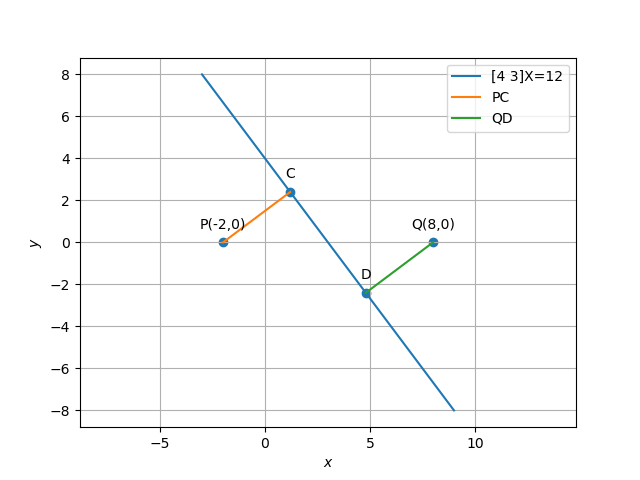
\includegraphics[width=0.75\columnwidth]{chapters/11/10/3/5/figs/line2}
	\end{center}
\caption{}
\label{fig:11/10/3/5/Fig1}
\end{figure}


